\documentclass[11pt]{article}

\usepackage[T1]{fontenc}
\usepackage[utf8]{inputenc}
\usepackage{lmodern}
\usepackage{amsmath,amssymb,amsthm,mathtools}
\usepackage{bm}
\usepackage{microtype}
\usepackage{booktabs}
\usepackage{array}
\usepackage{graphicx}
\usepackage{subcaption}
\usepackage{siunitx}
\usepackage{enumitem}
\usepackage{xcolor}
\usepackage[margin=1.15in]{geometry}
\usepackage[numbers,sort&compress]{natbib}
\usepackage[colorlinks=true,linkcolor=blue,citecolor=blue,urlcolor=blue]{hyperref}
\usepackage[nameinlink,noabbrev]{cleveref}

\bibliographystyle{abbrvnat}

\theoremstyle{plain}
\newtheorem{proposition}{Proposition}[section]
\newtheorem{theorem}[proposition]{Theorem}
\newtheorem{corollary}[proposition]{Corollary}
\newtheorem{lemma}[proposition]{Lemma}
\theoremstyle{definition}
\newtheorem{definition}[proposition]{Definition}
\theoremstyle{remark}
\newtheorem{remark}[proposition]{Remark}
\newtheorem{numericalresult}{Numerical Result}[section]

\newcommand{\R}{\mathbb{R}}
\newcommand{\mcC}{\mathcal{C}}
\newcommand{\mcJ}{\mathcal{J}}
\newcommand{\mcA}{\mathcal{A}}
\newcommand{\mustar}{\mu_\star}
\newcommand{\deltax}{\delta_\times}
\newcommand{\tr}{\operatorname{tr}}
\newcommand{\arcosh}{\operatorname{arcosh}}
\newcommand{\bigO}{\mathcal{O}}

\crefname{numericalresult}{Numerical Result}{Numerical Results}
\Crefname{numericalresult}{Numerical Result}{Numerical Results}

\title{Near-Degenerate Reversible \(1{:}2\) Resonance and Sextic Crossover in a \((2,3,5,7)\) Carnot Geodesic Flow}
\author{Gregorio Rozas Fernández\\\small Independent Researcher}
\date{September 18, 2026}

\begin{document}
\maketitle

\begin{abstract}
We study a reversible \(1{:}2\) resonance arising in the reduced normal geodesic flow of a rank-two Carnot structure with growth vector \((2,3,5,7)\). Reduction on generic coadjoint orbits and restriction to unit speed lead to the one-parameter system
\[
\dot x=\cos z,\qquad
\dot y=\sin z,\qquad
\dot z=-\frac12x^2+\frac12y^2-\mu,
\]
whose local Poincaré return is exact symplectic.

Along a symmetric periodic branch we numerically identify a resonance at which the complete monodromy matrix is consistent with
\[
DP_{\mu_\star}=-I.
\]
After fixing the linear symplectic normalization by the detuning and the reversing symmetry axes, the quartic interpolating Hamiltonian lies extremely close to the factorized form
\[
A(Q^2-P^2)^2.
\]
The resulting suppression of the quartic restoring term near the diagonal directions promotes the sixth-order Hamiltonian from a perturbative correction to a leading contribution.

This produces two distinct local period-two scales. The axial hyperbolic branches satisfy
\[
|\mcJ_H|\asymp\delta^2,
\]
whereas the near-diagonal elliptic branch exhibits the intermediate scaling
\[
|\mcJ_E|\asymp\delta^{3/2}
\]
in the regime
\[
\deltax\ll\delta\ll1.
\]

Because the quartic degeneracy is only approximate, the latter regime crosses over to a finite-amplitude plateau. Direct numerical solution of the exact second-return fixed-point equation at resonance reveals four nonzero fixed points, corresponding to two elliptic period-two cycles of the first return. Their action and Floquet scale agree closely with the sixth-order normal form.

After normalization by the intrinsic crossover scales, the leading scalar reduction yields coefficient-independent algebraic relations among amplitude, action, and stability. The results provide a concrete example of a near-degenerate reversible \(1{:}2\) resonance in which suppression of the quartic diagonal term promotes the sixth-order normal form and generates a measurable two-scale periodic-orbit geometry.
\end{abstract}

\section{Introduction}
\label{sec:introduction}

Resonances of area-preserving and reversible maps provide a natural setting in which local bifurcation theory, Hamiltonian normal forms, and periodic-orbit geometry interact. Among the simplest nontrivial cases is the \(1{:}2\) resonance, characterized by a double multiplier \(-1\) of the Poincaré return. At the resonant parameter, the square of the return is tangent to the identity, so that nonlinear terms determine the local organization of nearby periodic orbits.

Reversibility adds further structure. Symmetric periodic orbits intersect fixed sets of reversing involutions, and the corresponding symmetry lines provide a natural framework for locating and classifying bifurcating branches \cite{Sevryuk1986,LambRoberts1998}. In the area-preserving setting, normal forms near neutral multipliers \(+1\) and \(-1\) were studied systematically by Gelfreich and Gelfreikh \cite{GelfreichGelfreikh2010}. Near a semisimple multiplier \(-1\), the return admits a formal odd normal form, so that after changing sign one obtains a near-identity exact symplectic map described by an even interpolating Hamiltonian. Interpolating Hamiltonians have long been used to study resonant geometry and stability in conservative maps \cite{BazzaniEtAl1993}.

The system considered here arises from the normal geodesic flow of a rank-two, seven-dimensional Carnot structure with growth vector
\[
(2,3,5,7).
\]
The corresponding nilpotent algebra and its sub-Riemannian geodesic problem have previously appeared in the literature. In particular, Kruglikov, Vollmer, and Lukes-Gerakopoulos \cite{KruglikovVollmerLukesGerakopoulos2017} study the same structure, its coadjoint invariants, and questions of polynomial integrability. General background on sub-Riemannian extremals, left-invariant Hamiltonian systems, and coadjoint reduction may be found in \cite{AgrachevSachkov2004,AgrachevBarilariBoscain2019}.

Our starting point is therefore not a new Carnot algebra. The contribution begins with the reduced dynamics on its generic coadjoint orbits and, specifically, with a resonant periodic family that has not previously been analyzed in this form.

After rotational reduction, Carnot scaling, and restriction to unit speed, the geodesic equations reduce to
\begin{equation}
\boxed{
\dot x=\cos z,\qquad
\dot y=\sin z,\qquad
\dot z=-\frac12x^2+\frac12y^2-\mu.
}
\label{eq:intro-reduced-flow}
\end{equation}
The parameter \(\mu\) is the scale-invariant combination of the coadjoint Casimirs. The flow preserves volume and induces an exact symplectic local Poincaré map on the section \(x=0\).

Continuation of a primary symmetric periodic orbit numerically locates a \(1{:}2\) resonance at
\[
\mu=\mu_\star\simeq0.662869.
\]
At the corresponding parameter, the full monodromy matrix is numerically consistent with
\[
DP_{\mu_\star}=-I.
\]

The distinctive feature appears after fixing the linear canonical normalization by two pieces of information: the infinitesimal detuning and the tangent fixed sets of the two reversing involutions. In this fixed reversible chart the leading nonlinear Hamiltonian is
\[
H_4=A(Q^4+P^4)+BQ^2P^2.
\]
Writing
\[
\rho^2=2-\frac BA,
\]
we find
\[
\rho\simeq2.00118.
\]
The exactly quartic-degenerate value is \(\rho=2\), for which
\[
H_4=A(Q^2-P^2)^2.
\]

Thus the present system lies extremely close to a quartic degeneracy in which the diagonal directions are null directions of the leading nonlinear Hamiltonian. Define
\[
\sigma=4-\rho^2.
\]
Numerically,
\[
\sigma\simeq-4.73\times10^{-3}.
\]
The smallness of this coefficient promotes the sixth-order Hamiltonian
\[
H_6=dQ^6+eQ^4P^2+fQ^2P^4+gP^6
\]
to leading order in the near-diagonal sector.

The result is a two-scale local geometry. Along the axial directions,
\[
I_H\asymp\delta,\qquad |\mcJ_H|\asymp\delta^2.
\]
Near the almost-null diagonal directions, the leading scalar reduction is
\[
K_E(I)=-\delta I+A\sigma I^2+GI^3,
\qquad G=d+e+f+g>0,
\]
and in the regime
\[
\deltax\ll\delta\ll1
\]
one obtains
\[
I_E\asymp\delta^{1/2},
\qquad
|\mcJ_E|\asymp\delta^{3/2}.
\]

The \(3/2\) law is an intermediate asymptotic in the sense of scaling regimes lying between microscopic and ultimate asymptotic behavior \cite{Barenblatt1996}. Since \(\sigma<0\) is fixed, the branch ultimately crosses over to a finite-amplitude plateau as \(\delta\to0^+\). Direct numerical solution of the exact second-return equation at resonance reveals the corresponding residual elliptic period-two cycles.

The phenomenon considered here is distinct from the renormalization theory of repeated conservative period doubling \cite{GaidashevKoch2011}. We study a single semisimple local \(1{:}2\) resonance and the promotion of the sixth-order normal form caused by proximity to a quartic degeneracy; no period-doubling cascade or renormalization fixed point is assumed.

The novelty of the present work is therefore not the \((2,3,5,7)\) Carnot algebra itself, but the identification and analysis of a near-degenerate reversible \(1{:}2\) resonance in its reduced geodesic flow. The quartic near-degeneracy promotes the sixth-order normal form and produces two distinct periodic-orbit action scales together with a crossover to residual elliptic period-two cycles.

The exactly quartic-degenerate limit \(\sigma=0\) defines a separate higher-codimension problem and is not analyzed here.

\section{Geometric reduction and exact symplectic return}
\label{sec:reduction}

\subsection{Carnot model}

We consider the graded nilpotent Lie algebra with basis
\[
P,Q,K,V,U,Y,X
\]
and nonzero brackets
\[
[P,Q]=K,\qquad [P,K]=V,\qquad [Q,K]=U,
\]
\[
[P,U]=X,\qquad [P,V]=Y,\qquad [Q,U]=-Y,\qquad [Q,V]=X.
\]
Its growth vector is \((2,3,5,7)\).

The horizontal distribution is generated by \(P,Q\), taken orthonormal, so the normal Hamiltonian on the dual algebra is
\[
\mathcal H=\frac12(h_1^2+h_2^2).
\]
The complete Casimir calculation and canonical realization are given in \cref{app:lie}.

\subsection{Coadjoint reduction}

Let \((\xi,\eta)\) be the central momentum coordinates. On the generic stratum
\[
r^2=\xi^2+\eta^2>0,
\]
the third independent Casimir is
\[
\mathcal C
=
\kappa(\xi^2+\eta^2)
-\frac12(v^2-u^2)\eta
-vu\xi.
\]

Using the rotational automorphism, choose
\[
\xi=r,\qquad \eta=0.
\]
After Carnot scaling, the orbit family depends only on
\begin{equation}
\boxed{
\mu=\frac{\mathcal C}{r^{5/2}}.
}
\label{eq:mu-def}
\end{equation}

In canonical coordinates \((u,v,\Pi_u,\Pi_v)\), the reduced Hamiltonian is
\begin{equation}
\boxed{
H_\mu
=
\frac12
\left[
\Pi_u^2+
\left(
\Pi_v-\mu u-\frac12u^2v
\right)^2
\right].
}
\label{eq:reduced-H}
\end{equation}

On the unit-speed level,
\[
\dot u=\cos\phi,\qquad
\dot v=\sin\phi,\qquad
\dot\phi=-(\mu+uv).
\]

With
\[
x=\frac{u+v}{\sqrt2},\qquad
y=\frac{v-u}{\sqrt2},\qquad
z=\phi-\frac{\pi}{4},
\]
we obtain
\begin{equation}
\boxed{
\dot x=\cos z,\qquad
\dot y=\sin z,\qquad
\dot z=-\frac{x^2}{2}+\frac{y^2}{2}-\mu.
}
\label{eq:reduced-flow}
\end{equation}

\subsection{Reversibility and volume}

The flow admits the reversors
\[
\mathcal R_x(x,y,z)=(-x,y,-z),
\]
and
\[
\mathcal R_y(x,y,z)=(x,-y,\pi-z).
\]

It preserves
\[
\Omega=dx\wedge dy\wedge dz.
\]
A primitive of \(\iota_f\Omega\) is
\[
\alpha
=
-\cos z\,dx+
\left[
-\sin z-\frac{x^3}{6}
+x\left(\frac{y^2}{2}-\mu\right)
\right]dy,
\]
with
\[
d\alpha=\iota_f\Omega.
\]

\subsection{Local exact symplectic section}

Let
\[
X_\star=(0,y_\star,0)
\]
be the section point of the primary symmetric orbit. We use
\[
\Sigma=\{x=0,\cos z>0\}
\]
and a sufficiently small neighborhood \(U_\Sigma\) of \(X_\star\).

The return map
\[
P_\mu:U_\Sigma\to U_\Sigma
\]
is the \emph{local} return to this neighborhood. Intermediate crossings of the global plane \(x=0\) outside \(U_\Sigma\) are ignored.

Define
\begin{equation}
\boxed{
q=y-y_\star,\qquad p=\sin z.
}
\label{eq:exact-darboux}
\end{equation}
Then
\[
\omega_\Sigma=dq\wedge dp.
\]

With
\[
\lambda=q\,dp,
\]
the return is exact symplectic:
\begin{equation}
\boxed{
P_\mu^*\lambda-\lambda=dS_\mu.
}
\label{eq:return-exact}
\end{equation}

The exact action construction is developed in \cref{app:action}.

\section{The \texorpdfstring{\(1{:}2\)}{1:2} resonance and quartic near-degeneracy}
\label{sec:resonance}

\subsection{Symmetric primary periodic branch}

Starting from
\[
(0,a,0),
\]
reversibility reduces the periodic-orbit computation to the quarter-period conditions
\[
y(T_{1/4})=0,\qquad
z(T_{1/4})=\frac{\pi}{2}.
\]
Continuation in \(\mu\) produces a smooth primary branch.

\subsection{Numerical localization of the resonance}

The candidate \(1{:}2\) resonance is located by
\[
\tr DP_\mu(0)=-2.
\]
A multiprecision computation gives
\begin{equation}
\boxed{
\mustar
=0.66286900693051012809369086386036365\ldots.
}
\label{eq:mu-star}
\end{equation}
At 120-digit working precision, with an independent high-order Taylor integration of the state and variational equations, the complete event-corrected monodromy satisfies
\[
\|DP_{\mustar}(0)+I\|_F\simeq6.24\times10^{-47},
\]
while
\[
|\det DP_{\mustar}(0)-1|\simeq1.89\times10^{-49}.
\]
The resonance is therefore numerically identified as semisimple.  We summarize this as
\begin{equation}
\boxed{
DP_{\mustar}(0)=-I
}
\label{eq:resonance}
\end{equation}
within the quoted numerical accuracy.  The critical second return
\[
F_0=P_{\mustar}^2
\]
accordingly satisfies \(DF_0(0)=I\) to the same accuracy.

\subsection{Reversibility on the section}

The first reversor induces
\[
r(q,p)=(q,-p).
\]
A complementary reversing involution is generated by
\[
s_\mu=P_\mu r.
\]
Their tangent fixed sets at resonance define two complementary canonical directions. These directions fix the remaining rotational freedom after detuning normalization.

\subsection{Intrinsic detuning}

On the elliptic side define
\[
\delta(\mu)
=
\arccos\left(-\frac{\tr DP_\mu(0)}{2}\right)\ge0.
\]

Let
\[
M_\mu=-P_\mu.
\]
The orientation of \(\delta\) is chosen so that
\[
DM_\mu(0)
=
I+\delta
\begin{pmatrix}
0&-1\\
1&0
\end{pmatrix}
+\bigO(\delta^2).
\]

With
\[
\omega=dQ\wedge dP,\qquad
\iota_{X_H}\omega=dH,
\]
the quadratic generator is
\begin{equation}
\boxed{
H_2=-\delta I,\qquad
I=\frac{Q^2+P^2}{2}.
}
\label{eq:H2}
\end{equation}

\subsection{Reversible linear normalization}

The detuning determines the anisotropic symplectic scale
\[
q=\sqrt{\alpha_{\rm lin}}\,Q,\qquad
p=\frac{P}{\sqrt{\alpha_{\rm lin}}},
\]
with
\[
\alpha_{\rm lin}\simeq0.0946271414514.
\]

The remaining canonical rotations commuting with the normalized linear generator are removed by aligning the \(Q\)- and \(P\)-axes with the tangent fixed sets of the two reversing involutions. The reversible chart is then fixed up to discrete sign changes and interchange of the axes.

If the pure quartic coefficients before the intrinsic scaling are \(a_4q^4+c_4p^4\), the independent balancing scale is
\[
\alpha_{\rm bal}
=
\left(\frac{c_4}{a_4}\right)^{1/4}.
\]
Numerically,
\[
\alpha_{\rm bal}\simeq\alpha_{\rm lin}
\]
to relative order \(10^{-11}\).

\subsection{Odd resonant normal form}

At resonance,
\[
P_\star(w)=-w+\bigO(|w|^2).
\]
We fix the nonlinear gauge by using only the nonresonant canonical generators required to remove the even map terms: a cubic Hamiltonian generator eliminates the quadratic map term and a quintic generator eliminates the quartic map term. No resonant quartic Hamiltonian generator is added. The resulting canonical near-identity transformation puts the map into the odd form
\[
\widetilde P(w)
=
-w+\widetilde P_3(w)+\widetilde P_5(w)+\bigO(|w|^7).
\]

Define
\[
M=-\widetilde P.
\]
Then
\[
M
=
I+M_3+M_5+\bigO(7)
=
\exp(X_H),
\]
with
\[
H=H_4+H_6+\bigO(8).
\]
The extraction is detailed in \cref{app:normal-form}.

\subsection{Quartic interpolating Hamiltonian}

In the fixed reversible chart,
\begin{equation}
\boxed{
H_4
=
A(Q^4+P^4)+BQ^2P^2.
}
\label{eq:H4}
\end{equation}
The currently extracted values are approximately
\[
A\simeq203.6723580,\qquad B\simeq-408.3087120.
\]

Define
\begin{equation}
\boxed{
\rho^2=2-\frac BA.
}
\label{eq:rho-def}
\end{equation}
Then
\[
\rho\simeq2.001182918,
\]
and
\begin{equation}
\boxed{
\sigma=4-\rho^2\simeq-4.7330723\times10^{-3}.
}
\label{eq:sigma-def}
\end{equation}

At \(\rho=2\),
\[
H_4=A(Q^2-P^2)^2.
\]

In polar variables
\[
Q=\sqrt{2I}\cos\theta,\qquad
P=\sqrt{2I}\sin\theta,
\]
one obtains
\[
H_4
=
4AI^2-A\rho^2I^2\sin^22\theta.
\]
Hence
\[
H_4^{\rm ax}=4AI^2,
\]
whereas along an exact diagonal,
\[
H_4^{\rm diag}=A\sigma I^2.
\]

The quartic term is therefore fully active on the axes but strongly suppressed near the diagonals.

\section{Sextic promotion and two period-two scales}
\label{sec:sextic}

\subsection{Sixth-order interpolating Hamiltonian}

The next term is
\begin{equation}
\boxed{
H_6
=
dQ^6+eQ^4P^2+fQ^2P^4+gP^6.
}
\label{eq:H6}
\end{equation}
Define
\begin{equation}
\boxed{
G=d+e+f+g.
}
\label{eq:G-def}
\end{equation}

The detuned truncated normal form is
\begin{equation}
\boxed{
K_\delta
=
-\delta I+H_4+H_6
+
\bigO(\delta^2I,\delta I^2,I^4).
}
\label{eq:K-detuned}
\end{equation}

\subsection{Axial hyperbolic branches}

On the \(Q\)-axis,
\[
K_Q
=
-\delta I+4AI^2+8dI^3+\cdots.
\]
Hence
\[
I_Q
=
\frac{\delta}{8A}
-
\frac{3d}{64A^3}\delta^2
+
\bigO(\delta^3),
\]
and
\begin{equation}
\boxed{
\mcJ_Q
=
-\frac{\delta^2}{16A}
+
\frac{d}{64A^3}\delta^3
+
\bigO(\delta^4).
}
\label{eq:JQ}
\end{equation}

Similarly,
\begin{equation}
\boxed{
\mcJ_P
=
-\frac{\delta^2}{16A}
+
\frac{g}{64A^3}\delta^3
+
\bigO(\delta^4).
}
\label{eq:JP}
\end{equation}
Therefore
\begin{equation}
\boxed{
|\mcJ_H|\asymp\delta^2.
}
\label{eq:axial-action}
\end{equation}

The physical second-return exponents satisfy
\begin{equation}
\boxed{
\kappa_{F,Q}
=
2\rho\delta
+
\frac{3d-e}{4A^2\rho}\delta^2
+
\bigO(\delta^3),
}
\label{eq:kappaQ}
\end{equation}
and
\begin{equation}
\boxed{
\kappa_{F,P}
=
2\rho\delta
+
\frac{3g-f}{4A^2\rho}\delta^2
+
\bigO(\delta^3).
}
\label{eq:kappaP}
\end{equation}

\subsection{Near-diagonal scalar reduction}

Along the exact diagonal, \(Q^2=P^2=I\), so the leading scalar model is
\begin{equation}
\boxed{
K_E(I)
=
-\delta I+aI^2+GI^3,
\qquad
a=A\sigma<0.
}
\label{eq:diagonal-scalar}
\end{equation}

The positive stationary solution is
\begin{equation}
\boxed{
I_E
=
\frac{|a|+\sqrt{a^2+3G\delta}}{3G}.
}
\label{eq:IE}
\end{equation}

Define
\begin{equation}
\boxed{
\deltax=\frac{a^2}{G}.
}
\label{eq:crossover-scale}
\end{equation}

For \(\delta\gg\deltax\),
\[
I_E\sim\sqrt{\frac{\delta}{3G}},
\qquad
r_E\asymp\delta^{1/4}.
\]

The reduced action is
\[
\mcJ_E=-aI_E^2-2GI_E^3,
\]
so
\begin{equation}
\boxed{
\mcJ_E
\sim
-\frac{2}{3^{3/2}\sqrt G}\delta^{3/2}.
}
\label{eq:elliptic-action-scaling}
\end{equation}

\subsection{Two-scale periodic-orbit geometry}

The axial scale is
\[
r_H\asymp\delta^{1/2},
\]
whereas the near-diagonal scale is
\[
r_E\asymp\delta^{1/4}.
\]
Hence
\[
\frac{r_E}{r_H}\asymp\delta^{-1/4}.
\]

Invariantly,
\[
\boxed{
|\mcJ_H|\asymp\delta^2,
\qquad
|\mcJ_E|\asymp\delta^{3/2}.
}
\]

\subsection{Breakdown of the outer scaling}

Because \(a<0\) is fixed, the sextic power law cannot persist to \(\delta=0\). Instead,
\[
I_E\to I_0^{\rm scalar}
=
\frac{2|a|}{3G},
\]
and
\[
\mcJ_E\to
\mcJ_0^{\rm scalar}
=
-\frac{4|a|^3}{27G^2}.
\]
The next section describes this crossover.

\section{Quartic--sextic crossover}
\label{sec:crossover}

\subsection{Intrinsic crossover variable}

Define
\[
\boxed{
u=\frac{\delta}{\deltax}\ge0.
}
\]
Let
\[
R(u)=\frac{1+\sqrt{1+3u}}{2}.
\]
Then the scalar model gives
\begin{equation}
\boxed{
\frac{I_E}{I_0^{\rm scalar}}
=
R(u).
}
\label{eq:R-crossover}
\end{equation}

\subsection{Normalized action crossover}

Using the scalar residual action,
\begin{equation}
\boxed{
\frac{\mcJ_E}{\mcJ_0^{\rm scalar}}
=
4R^3-3R^2.
}
\label{eq:action-crossover}
\end{equation}

For \(u\gg1\), this reproduces the \(3/2\) action law. For \(u\to0\), the normalized scalar action tends to one.

\subsection{Effective action exponent}

Define
\[
\nu_{\mcJ}
=
\frac{d\log|\mcJ_E|}{d\log\delta}.
\]
The scalar model gives
\[
\boxed{
\nu_{\mcJ}
=
\frac{3(\sqrt{1+3u}-1)}
{2\sqrt{1+3u}-1}.
}
\]
Thus
\[
\nu_{\mcJ}\to\frac32
\quad(u\to\infty),
\qquad
\nu_{\mcJ}\to0
\quad(u\to0).
\]

\subsection{Leading Floquet crossover}

Near the diagonal,
\[
H_4
=
aI^2+4A\rho^2I^2x^2+\cdots.
\]
The physical second-return angle predicted by the scalar reduction is
\begin{equation}
\boxed{
\vartheta_F
=
8\rho I_E
\sqrt{
A\sqrt{a^2+3G\delta}
}.
}
\label{eq:thetaF}
\end{equation}

At \(\delta=0\),
\[
\vartheta_0^{\rm scalar}
=
8\rho I_0^{\rm scalar}\sqrt{A|a|}.
\]
Thus
\[
\boxed{
\frac{\vartheta_F}{\vartheta_0^{\rm scalar}}
=
R\sqrt{2R-1}.
}
\]

For \(u\gg1\),
\[
\vartheta_F\asymp\delta^{3/4}.
\]

\subsection{Parameter-free scalar relations}

Define
\[
X=\frac{I_E}{I_0^{\rm scalar}},
\qquad
Y=\frac{\mcJ_E}{\mcJ_0^{\rm scalar}},
\qquad
Z=\frac{\vartheta_F}{\vartheta_0^{\rm scalar}}.
\]
Within the scalar reduction,
\begin{equation}
\boxed{
Y=4X^3-3X^2,
}
\label{eq:YX}
\end{equation}
and
\begin{equation}
\boxed{
Z=X\sqrt{2X-1}.
}
\label{eq:ZX}
\end{equation}

These are coefficient-independent scalar crossover relations, not exact identities of the complete return-map germ.

\subsection{Corrections beyond the scalar reduction}

The complete sixth-order Hamiltonian is anisotropic:
\[
d\neq g,\qquad e\neq f.
\]
Therefore the true residual equilibrium is shifted slightly away from the exact diagonal. The scalar crossover curves should consequently be interpreted as leading normalized predictions. Their deviations measure angular sixth-order structure and higher-order terms.

\section{Numerical validation and orbital reconstruction}
\label{sec:numerics}

\subsection{Numerical strategy}

The numerical tests are based on the exact local return of the reduced flow.  Critical-jet predictions are fixed before comparison with periodic-orbit observables.  The action is evaluated from the exact section formula
\[
\mcJ=\frac12\int_\Gamma(F^*\lambda-\lambda),
\qquad \lambda=q\,dp,
\]
so that the very small residual actions do not require subtraction of two large flow integrals.  The implementation and convergence diagnostics are described in \cref{app:numerics}.

\subsection{Multiprecision localization of the resonant primary orbit}

A dedicated high-order Taylor integrator was used to repeat the resonance computation in arbitrary precision.  The trigonometric state equations and the variational equations are advanced by recursively generated Taylor coefficients, so the calculation does not rely on double-precision ODE arithmetic.

The refined resonant parameter is
\begin{equation}
\boxed{
\mu_\star
=0.66286900693051012809369086386036365\ldots
}
\label{eq:mustar-mp}
\end{equation}
with
\[
y_\star
=-2.57258930747694896652177432487053\ldots,
\]
\[
T_{1/4,\star}
=3.01795545336085961004746139780291\ldots.
\]

At 120-digit working precision, using a Taylor order of 38 and maximal step size $0.05$, the complete event-corrected monodromy satisfies
\[
\boxed{
\|DP_{\mu_\star}+I\|_F
\simeq 6.24\times10^{-47},
}
\]
while
\[
|\det DP_{\mu_\star}-1|
\simeq1.89\times10^{-49}.
\]
The residual off-diagonal entries are at the $10^{-47}$ scale or smaller.  This convergence of the complete matrix, rather than the trace alone, is the numerical basis for identifying the resonance as semisimple.

\subsection{Independent critical-jet re-extraction}

The complete fifth-order return jet was re-extracted independently in multiprecision by transporting a bivariate polynomial jet in the section variables $(q,p)$ through the Taylor integrator.  The variable return time is then solved formally, degree by degree, from the implicit event equation $x(T_\star+\tau(q,p),q,p)=0$.  This avoids polynomial regression of sampled map values.

The nonlinear oddification is fixed by the nonresonant gauge described in \cref{app:normal-form}: a cubic Hamiltonian generator removes the quadratic map term and a quintic generator removes the quartic map term, with no additional resonant quartic generator.  Two independent transports, using $h_{\max}=0.22$ at 55-digit working precision and $h_{\max}=0.20$ at 60-digit working precision, give a stable sextic plateau.

The linear and quartic balancing scales are
\[
\boxed{
\alpha_{\rm lin}=0.0946271414514,\qquad
\alpha_{\rm bal}=0.0946271414515,
}
\]
with relative discrepancy approximately $1.2\times10^{-12}$.  In the fixed reversible chart the re-extracted coefficients are
\[
A=203.6723580,\qquad B=-408.3087120,
\]
\[
\rho=2.001182918,\qquad
\sigma=-4.7330723\times10^{-3},
\]
and
\[
d=27009.26240,\qquad e=271555.83499,
\]
\[
f=512441.22879,\qquad g=75140.77917.
\]
Hence
\[
\boxed{
G=886147.10535,\qquad
\Delta_6=-289016.91057.
}
\]
The two jet discretizations differ by only $3.0\times10^{-6}$ in $d$, $1.8\times10^{-5}$ in $e$, $1.6\times10^{-5}$ in $f$, and $1.6\times10^{-7}$ in $g$ in absolute units; the resulting values of $G$ differ by $1.4\times10^{-6}$.  The corresponding scalar crossover scale is
\[
\deltax\simeq1.0486840\times10^{-6}.
\]
These quantities are fixed before comparison with the periodic-orbit observables below.

\subsection{Axial action law and orbital quartic calibration}

The leading axial normal form predicts
\[
\mcJ_H=-\frac{\delta^2}{16A}+\bigO(\delta^3),
\]
so that
\begin{equation}
\boxed{
A_{\rm orb}(\delta)
=-\frac{\delta^2}{16\bar{\mcJ}},
\qquad
\bar{\mcJ}=\frac{\mcJ_Q+\mcJ_P}{2}.
}
\label{eq:Aorb}
\end{equation}
The physical second-return exponents similarly give
\begin{equation}
\boxed{
\rho_{\rm orb}(\delta)
=
\frac{\kappa_{F,Q}+\kappa_{F,P}}{4\delta}.
}
\label{eq:rhoorb}
\end{equation}

The exact-return results from two interlaced dyadic ladders are shown in \cref{tab:orbital-quartic}.  The raw estimators approach the critical-jet values monotonically as $\delta$ decreases.

\begin{table}[t]
\centering
\caption{Orbital reconstruction of the leading quartic coefficients from exact axial period-two orbits.}
\label{tab:orbital-quartic}
\begin{tabular}{ccc}
\toprule
$\delta$ & $A_{\rm orb}$ & $\rho_{\rm orb}$ \\
\midrule
$2.0\times10^{-2}$ & $202.35030$ & $2.0103251$ \\
$1.0\times10^{-2}$ & $203.00736$ & $2.0058993$ \\
$5.0\times10^{-3}$ & $203.33850$ & $2.0035771$ \\
$1.6\times10^{-2}$ & $202.61225$ & $2.0085900$ \\
$8.0\times10^{-3}$ & $203.13954$ & $2.0049791$ \\
$4.0\times10^{-3}$ & $203.40492$ & $2.0031040$ \\
\bottomrule
\end{tabular}
\end{table}

First Richardson extrapolation gives, on the successive pairs of the two ladders,
\[
A_{\rm orb}^{[1]}
=203.66441,
\ 203.66964,
\ 203.66683,
\ 203.67029,
\]
and
\[
\rho_{\rm orb}^{[1]}
=2.0014734,
\ 2.0012549,
\ 2.0013681,
\ 2.0012289.
\]
These values converge toward
\[
A_{\rm jet}=203.6723580,
\qquad
\rho_{\rm jet}=2.001182918.
\]
Thus the quartic balance, and in particular the proximity to $\rho=2$, is visible directly in invariant periodic-orbit observables rather than only in the fitted return jet.

\subsection{Why the subleading axial coefficients do not isolate the critical sextic jet}
\label{sec:axial-contamination}

The numerical campaign also exposes an important limitation of the simpler axial reconstruction proposed at an earlier stage of the analysis.  The detuned normal form has the structure
\begin{equation}
K_\delta
=
-\delta I
+H_4
+H_6
+\delta\,H_{4,1}
+\gamma\delta^2 I
+\cdots,
\label{eq:detuned-extended}
\end{equation}
where $H_{4,1}$ is a detuning-dependent quartic polynomial.  On an axial branch, $I=\bigO(\delta)$, and therefore
\[
H_6=\bigO(\delta^3),
\qquad
\delta H_{4,1}=\bigO(\delta^3),
\qquad
\delta^2 I=\bigO(\delta^3).
\]
Consequently, the $\delta^3$ action coefficient and the $\delta^2$ Floquet correction contain both the critical sextic jet and detuning-dependent lower-order terms.  They cannot be used to reconstruct $d,e,f,g$ from the critical map alone unless the parameter-dependent normal form is computed to the same order.

This is confirmed by the exact-return data: the two axial families have the correct common leading law $2\rho\delta$, but their measured subleading Floquet corrections do not agree with formulas containing only the critical coefficients $d,e,f,g$.  We therefore use the axial branches only for the robust leading reconstruction of $A$ and $\rho$.  No sextic coefficient is inferred from the contaminated subleading axial channel in the final analysis.

\subsection{Elliptic action reconstruction of \texorpdfstring{$G$}{G}}

The near-diagonal branch provides a cleaner test of the sextic coefficient.  Within the scalar reduction,
\[
3\mcJ_E=aI^2-2\delta I,
\]
so the physical positive root is
\[
I
=
\frac{
\delta-\sqrt{\delta^2+3a\mcJ_E}
}{a},
\]
and
\begin{equation}
\boxed{
G_{\rm ell}
=
\frac{\delta-2aI}{3I^2}.
}
\label{eq:Gell}
\end{equation}

The reconstruction is remarkably stable throughout the inner crossover region.  Representative values are
\begin{table}[t]
\centering
\caption{Elliptic action reconstruction of $G$.  The fixed critical-jet target is $G_{\rm jet}=8.8614711\times10^5$.}
\label{tab:Gell}
\begin{tabular}{ccc}
\toprule
$u=\delta/\deltax$ & $G_{\rm ell}$ & relative difference from $G_{\rm jet}$ \\
\midrule
$0$    & $8.85903\times10^5$ & $-2.8\times10^{-4}$ \\
$0.01$ & $8.86023\times10^5$ & $-1.4\times10^{-4}$ \\
$0.1$  & $8.85904\times10^5$ & $-2.8\times10^{-4}$ \\
$1$    & $8.85186\times10^5$ & $-1.1\times10^{-3}$ \\
$10$   & $8.82339\times10^5$ & $-4.3\times10^{-3}$ \\
$100$  & $8.73139\times10^5$ & $-1.47\times10^{-2}$ \\
\bottomrule
\end{tabular}
\end{table}
The gradual outer drift is consistent with higher-order corrections becoming more visible as the branch leaves the local crossover scale.

\subsection{Residual elliptic period-two cycles at resonance}

At $\mu=\mu_\star$, direct multiprecision solution of
\[
F(q,p)=(q,p)
\]
finds the nonzero residual period-two cycles predicted by the sixth-order normal form.  One representative fixed point of $F$ is
\[
\boxed{
(q,p)
=
(2.56839185346349\times10^{-4},
 2.83395697372187\times10^{-3})
}
\]
and its first-return companion is
\[
P(q,p)
=
(-2.67259191745878\times10^{-4},
 -2.70365354787740\times10^{-3}).
\]
The second symmetry-related cycle supplies the other two nonzero fixed points of $F$.

The physical second-return Floquet angle is
\[
\boxed{
\vartheta_F
=1.62684506536\times10^{-4},
}
\]
with
\[
\tr DF
=1.99999997353375139\ldots,
\]
and the multiprecision determinant error is below $10^{-23}$ in this computation.

The exact reduced symplectic action is
\begin{equation}
\boxed{
\mcJ_0^{\rm exact}
=-1.69102354131\times10^{-13}.
}
\label{eq:residual-action-exact}
\end{equation}
For comparison, the scalar prediction is
\[
\mcJ_0^{\rm scalar}
=-1.69009171482\times10^{-13},
\]
while the sixth-order polynomial prediction is approximately
\[
\mcJ_0^{(6)}
=-1.69021\times10^{-13}.
\]
The residual exact action is therefore already reproduced at the $10^{-3}$ level by the frozen sixth-order description.

\subsection{Direct quartic--sextic crossover}
\label{sec:numerical-crossover}

The exact elliptic family was continued through
\[
u=0,\ 0.01,\ 0.03,\ 0.1,\ 0.3,\ 1,\ 3,\ 10,\ 30,\ 100.
\]
The branch was selected by continuation from the residual cycle together with the sixth-order predictor; this avoids numerical jumps to the coexisting axial fixed points at the largest detunings.

For the invariant normalized action and Floquet angle,
\[
Y=\frac{\mcJ_E}{\mcJ_0^{\rm scalar}},
\qquad
Z=\frac{\vartheta_F}{\vartheta_0^{\rm scalar}},
\]
the exact-return data closely follow the coefficient-independent scalar curves
\[
Y_{\rm sc}=4R^3-3R^2,
\qquad
Z_{\rm sc}=R\sqrt{2R-1}.
\]
Representative comparisons are shown in \cref{tab:crossover-data}.

\begin{table}[t]
\centering
\caption{Exact-return crossover compared with the scalar prediction.}
\label{tab:crossover-data}
\begin{tabular}{ccccc}
\toprule
$u$ & $Y$ & $Y_{\rm sc}$ & $Z$ & $Z_{\rm sc}$ \\
\midrule
$0$    & $1.00055$ & $1.00000$ & $0.99997$ & $1.00000$ \\
$0.01$ & $1.04545$ & $1.04517$ & $1.01494$ & $1.01492$ \\
$0.1$  & $1.46679$ & $1.46611$ & $1.14267$ & $1.14263$ \\
$1$    & $6.75730$ & $6.74997$ & $2.12186$ & $2.12132$ \\
$10$   & $109.605$ & $109.300$ & $7.75513$ & $7.74866$ \\
$30$   & $504.342$ & $502.040$ & $16.2990$ & $16.2759$ \\
$100$  & $2859.51$ & $2836.57$ & $38.3127$ & $38.2148$ \\
\bottomrule
\end{tabular}
\end{table}

Across this entire range the normalized action differs from the scalar curve by less than $0.81\%$, and the normalized Floquet angle by less than $0.52\%$.  The data therefore connect the residual plateau continuously to the outer sextic regime without any fitted crossover parameter.

The independent critical-jet audit also reconstructs the nonlinear canonical chart.  Writing
\[
I_{\rm NF}=\frac{Q^2+P^2}{2},
\qquad
X=\frac{I_{\rm NF}}{I_0^{\rm scalar}},
\]
the exact-return amplitude follows the scalar prediction $X_{\rm sc}=R(u)$ to within $0.62\%$ over the full range $0\le u\le100$.  At the residual cycle, $X=1.00037$, a deviation of only $0.037\%$ from the scalar plateau.  Reconstructing the canonical map with the two independent jet discretizations changes $I_{\rm NF}$ by at most $4.0\times10^{-13}$ relatively across the entire crossover.  The first-return companion points have equal $I_{\rm NF}$ to relative accuracy better than $7\times10^{-6}$ even at $u=100$.

\begin{figure}[t]
\centering
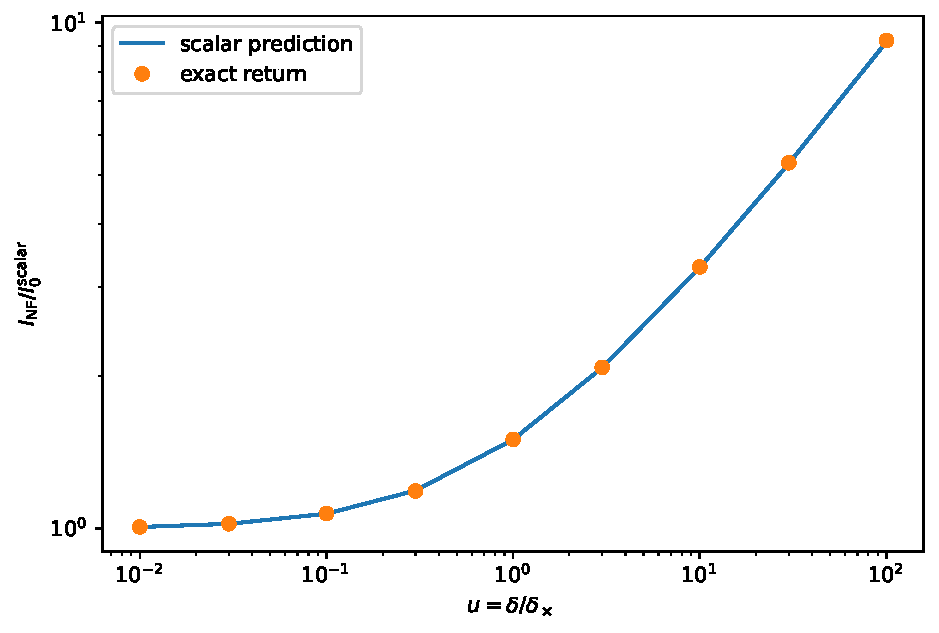
\includegraphics[width=.72\linewidth]{figures/fig06_amplitude_crossover.pdf}
\caption{Normal-form amplitude across the quartic--sextic crossover.  Exact-return fixed points are transformed with the independently reconstructed critical canonical chart.  The continuous curve is the coefficient-independent scalar prediction $X=R(u)$; no amplitude normalization is fitted to the continuation data.}
\label{fig:amplitude-crossover}
\end{figure}

Eliminating $u$ gives an additional parameter-free test.  The exact data remain close to
\[
Y=4X^3-3X^2,\qquad Z=X\sqrt{2X-1}.
\]
The maximum relative departures over the computed range are about $1.1\%$ in the action relation and $0.7\%$ in the Floquet relation.

\begin{figure}[t]
\centering
\begin{subfigure}{.48\linewidth}
\centering
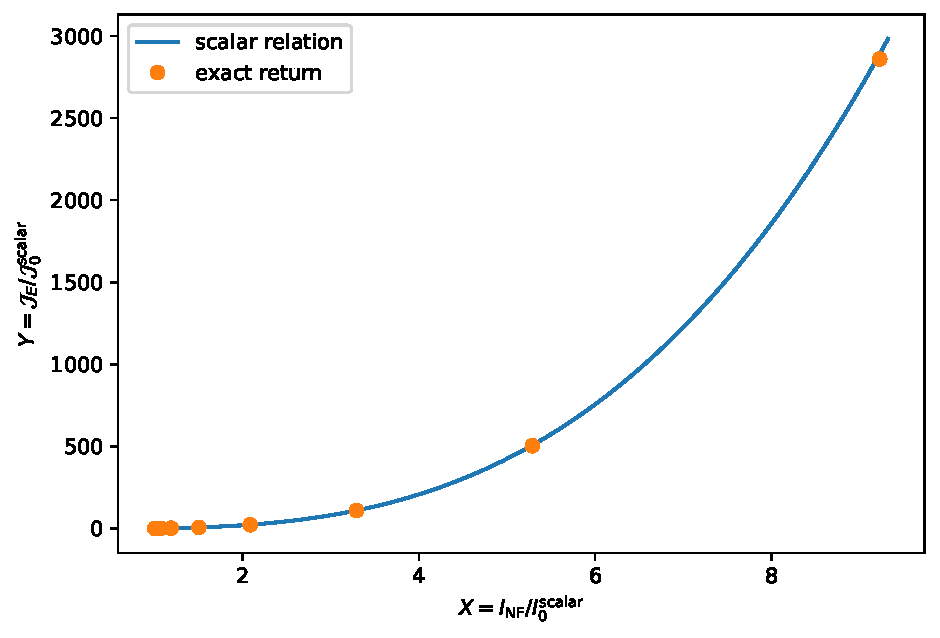
\includegraphics[width=\linewidth]{figures/fig08_action_vs_amplitude.pdf}
\caption{Action--amplitude relation.}
\end{subfigure}
\hfill
\begin{subfigure}{.48\linewidth}
\centering
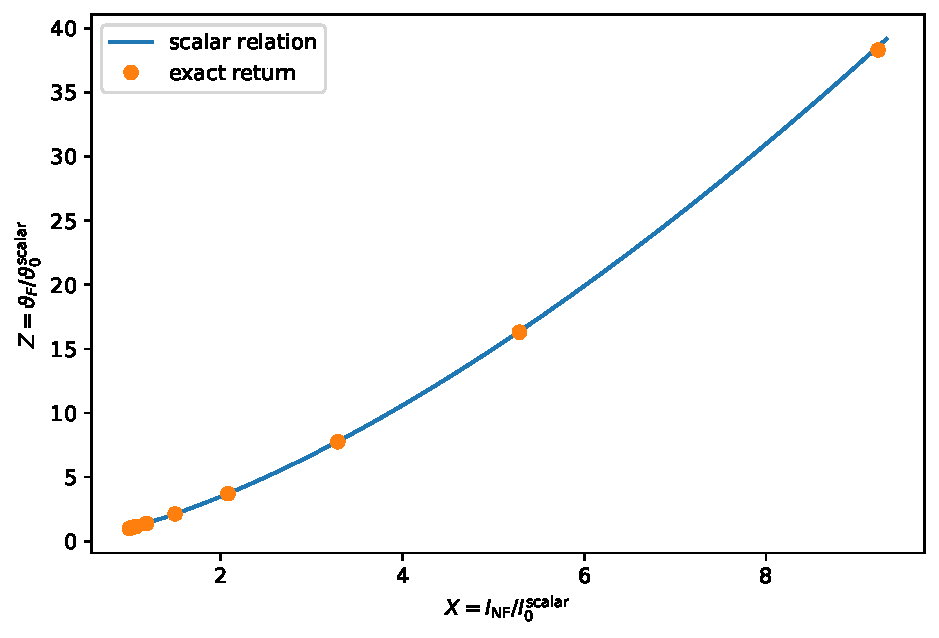
\includegraphics[width=\linewidth]{figures/fig08_floquet_vs_amplitude.pdf}
\caption{Floquet--amplitude relation.}
\end{subfigure}
\caption{Parameter-free crossover tests after eliminating the continuation parameter.  The curves are the scalar relations; the markers are exact-return observables in the reconstructed canonical chart.}
\label{fig:parameter-free}
\end{figure}

\subsection{Effective exponents}

Local logarithmic slopes extracted from neighboring continuation points track the scalar effective exponents.  For example, near $u=1$ the discrete data give
\[
\nu_{\mcJ}\simeq0.968,
\qquad
\nu_\vartheta\simeq0.426,
\]
compared with the scalar values
\[
1,
\qquad
\frac7{16}=0.4375.
\]
By $u=30$ the agreement is much tighter:
\[
\nu_{\mcJ}\simeq1.41646
\quad\text{versus}\quad
1.41703,
\]
\[
\nu_\vartheta\simeq0.69375
\quad\text{versus}\quad
0.69484.
\]
The observed drift toward $3/2$ and $3/4$ confirms the intermediate-asymptotic interpretation rather than a fixed power law extending to resonance.


\begin{figure}[t]
\centering
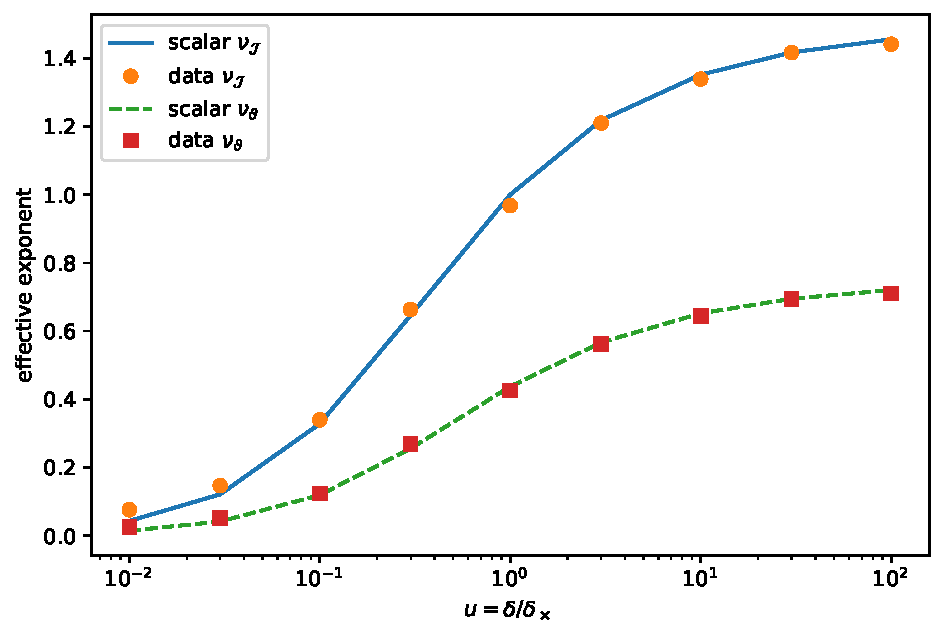
\includegraphics[width=.72\linewidth]{figures/fig07_effective_exponents.pdf}
\caption{Effective action and Floquet exponents across the exact-return crossover, compared with the scalar prediction.}
\label{fig:effective-exponents}
\end{figure}

\begin{figure}[t]
\centering
\begin{subfigure}{.48\linewidth}
\centering
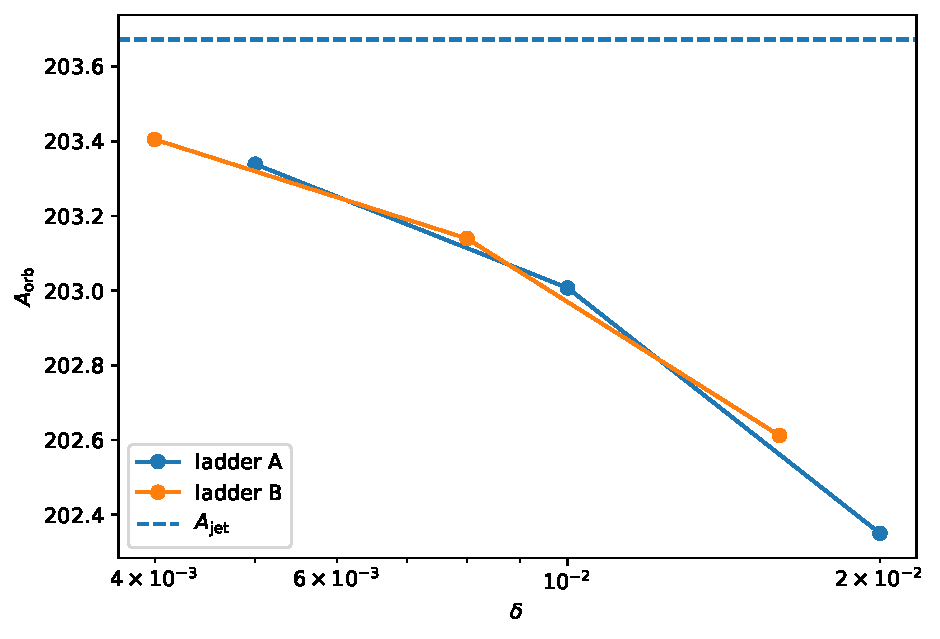
\includegraphics[width=\linewidth]{figures/fig09_Aorb.pdf}
\caption{Orbital reconstruction of $A$.}
\end{subfigure}
\hfill
\begin{subfigure}{.48\linewidth}
\centering
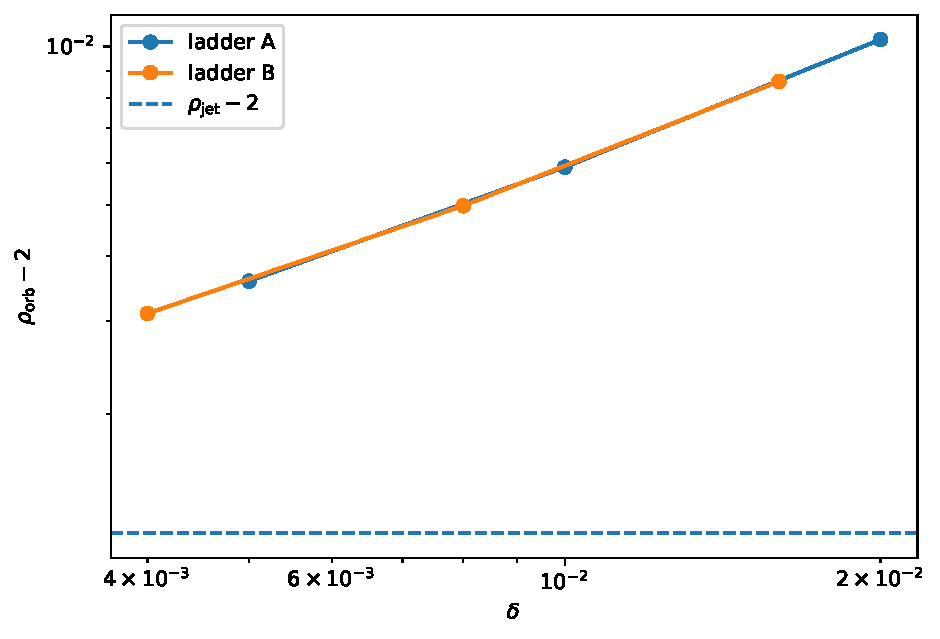
\includegraphics[width=\linewidth]{figures/fig09_rhoorb_minus2.pdf}
\caption{Orbital reconstruction of $\rho-2$.}
\end{subfigure}
\caption{Leading quartic coefficients reconstructed from exact axial action and Floquet observables.  Horizontal reference lines are fixed by the independent critical-jet extraction.}
\label{fig:orbital-quartic}
\end{figure}

\subsection{Numerical status}

The following parts of the numerical program are now complete:
\begin{itemize}[leftmargin=2em]
\item multiprecision localization and semisimplicity audit of the $1{:}2$ resonance;
\item independent multiprecision transport of the complete critical fifth-order return jet;
\item canonical nonresonant oddification and reconstruction of $H_4$, $H_6$, and the nonlinear normal-form chart;
\item exact-return axial validation of the leading quartic coefficients $A$ and $\rho$;
\item multiprecision residual-cycle action and Floquet calculation;
\item exact-return crossover continuation from $u=0$ to $u=100$, including the normal-form amplitude $I_{\rm NF}$;
\item elliptic action reconstruction of the diagonal sextic coefficient $G$;
\item parameter-free amplitude--action and amplitude--Floquet crossover tests.
\end{itemize}

The campaign also shows that a sextic reconstruction from subleading axial coefficients alone is not justified without the detuning-dependent normal form in \eqref{eq:detuned-extended}; this claim has therefore been removed rather than fitted away.  The principal remaining extension is no longer required for the present conclusions: it would be the full parameter-dependent normal form through the weighted order needed to separate critical sextic and detuning-dependent contributions on the axial branches.

\section{Discussion}
\label{sec:discussion}

\subsection{Mechanism of sextic promotion}

The central feature of the resonance is not an unusually large sixth-order term by itself. It is the suppression of the quartic term in a distinguished angular sector.

Along the axes, the quartic Hamiltonian remains nondegenerate and yields the ordinary law
\[
|\mcJ_H|\asymp\delta^2.
\]

Near the diagonals, the coefficient of the quartic radial term is proportional to the small quantity
\[
\sigma=4-\rho^2.
\]
The sixth-order term therefore enters at leading order and generates the intermediate law
\[
|\mcJ_E|\asymp\delta^{3/2}.
\]

This is the sense in which the sextic term is dynamically promoted.

\subsection{Why the quartic balance is meaningful}

The quartic balance is not imposed by an arbitrary anisotropic rescaling. The detuning fixes the linear symplectic scale, and the reversing involutions fix the remaining rotational freedom.

An independently defined quartic balancing scale agrees numerically with the detuning scale to very high accuracy. The additional orbital reconstruction of \(A\) and \(\rho\) provides a second test of the same conclusion.

\subsection{Intermediate scaling and crossover}

For fixed
\[
\sigma<0,
\]
the \(3/2\) law is not the ultimate \(\delta\to0\) asymptotic. The correct interpretation is
\[
\deltax\ll\delta\ll1
\]
for the sextic-dominated regime, followed by a crossover to a finite-amplitude plateau.

The normalized scalar model provides a compact description of that transition.

\subsection{Residual elliptic cycles}

The negative sign of the quartic diagonal coefficient leads, in the sixth-order truncation, to nonzero elliptic equilibria at resonance. The exact second return numerically exhibits the corresponding residual period-two cycles.

Their existence, multiplicity, elliptic stability, action scale, and Floquet scale together provide a restrictive test of the sixth-order model.

\subsection{Observable accessibility of the normal form}

The leading axial action determines \(A\), while the leading physical second-return Floquet exponent determines \(\rho\).  These two limits are robust because the first detuning-dependent corrections enter only one order later, and the Richardson extrapolations converge toward the critical-jet values.

The numerical audit also clarifies what cannot be inferred from the same axial data.  At subleading order, the critical sextic Hamiltonian is mixed with detuning-dependent quartic terms and with quadratic corrections to the linear detuning; see \cref{sec:axial-contamination,app:axial-contamination}.  We therefore do not interpret the axial \(\delta^3\) action coefficients or \(\delta^2\) Floquet corrections as direct measurements of \(d,e,f,g\).

The diagonal sextic combination \(G\) is instead tested by the near-diagonal elliptic branch, for which the promoted sextic term enters asymptotically ahead of the first detuning-dependent quartic correction.  The observable hierarchy used in the final analysis is therefore
\[
\text{leading axial action}\longrightarrow A,
\]
\[
\text{leading axial Floquet exponent}\longrightarrow\rho,
\]
and
\[
\text{near-diagonal action--Floquet crossover}\longrightarrow G.
\]

The return jet and the periodic-orbit geometry remain complementary descriptions of the same resonant germ, but the comparison is made only at asymptotic orders where the relevant coefficient is identifiable.

\subsection{Model-dependent and coefficient-independent features}

The values of
\[
\mu_\star,A,B,d,e,f,g
\]
are specific to the present Carnot geodesic flow and the fixed reversible normal-form chart.

By contrast, once the scalar reduced Hamiltonian has the form
\[
-\delta I+aI^2+GI^3,
\qquad
a<0,\ G>0,
\]
the normalized relations
\[
Y=4X^3-3X^2
\]
and
\[
Z=X\sqrt{2X-1}
\]
are coefficient independent.

They should be regarded as leading scalar crossover relations, not as universal identities of arbitrary reversible \(1{:}2\) resonances.

\subsection{Scope}

The analysis is local in phase space. No conclusion about global integrability follows from the resonance alone.

Likewise, the exactly quartic-degenerate limit
\[
\sigma=0
\]
defines a different higher-codimension asymptotic problem. That limit is deliberately separated from the fixed-\(\sigma<0\) crossover studied here.

\section{Conclusions}
\label{sec:conclusions}

We have identified numerically a reversible \(1{:}2\) resonance in the reduced geodesic flow of a \((2,3,5,7)\) Carnot structure. The associated local Poincaré return is exact symplectic, and the complete resonant monodromy is numerically consistent with the semisimple matrix \(-I\).

In the reversible canonical chart fixed by the detuning and symmetry axes, the quartic interpolating Hamiltonian lies unusually close to
\[
A(Q^2-P^2)^2.
\]
This quartic near-degeneracy promotes the sixth-order Hamiltonian to leading order near the diagonal directions and generates two distinct local period-two action scales:
\[
|\mcJ_H|\asymp\delta^2,
\]
for the axial hyperbolic branches, and
\[
|\mcJ_E|\asymp\delta^{3/2},
\]
for the near-diagonal elliptic branch in the sextic-dominated intermediate regime.

Because the quartic unfolding is small but nonzero, the anomalous law crosses over to a finite-amplitude plateau. Direct numerical solution of the exact return at resonance reveals the corresponding residual elliptic period-two cycles, whose action and Floquet scale agree closely with the sixth-order model.

The resulting mechanism may be summarized schematically as
\[
\begin{gathered}
\text{\(1{:}2\) resonance}
\longrightarrow
\text{quartic near-degeneracy}
\longrightarrow
\text{sextic promotion}
\\[2mm]
\longrightarrow
\text{two-scale periodic-orbit dynamics}
\longrightarrow
\text{quartic--sextic crossover}.
\end{gathered}
\]

The exactly quartic-degenerate limit
\[
\sigma=0
\]
defines a separate higher-codimension asymptotic problem and is left for future work.


\appendix
\section{Lie--Poisson reduction and canonical realization}
\label{app:lie}

\subsection{Graded Lie algebra}

Let
\[
\mathfrak n
=
\operatorname{span}
\{P,Q,K,V,U,Y,X\}
\]
with nonzero brackets
\[
[P,Q]=K,
\]
\[
[P,K]=V,\qquad [Q,K]=U,
\]
\[
[P,U]=X,\qquad [P,V]=Y,
\]
\[
[Q,U]=-Y,\qquad [Q,V]=X.
\]

The grading is
\[
\mathfrak n_1=\operatorname{span}\{P,Q\},\quad
\mathfrak n_2=\operatorname{span}\{K\},
\]
\[
\mathfrak n_3=\operatorname{span}\{V,U\},\quad
\mathfrak n_4=\operatorname{span}\{Y,X\},
\]
so the growth vector is
\[
\boxed{(2,3,5,7).}
\]

Equivalently,
\[
[P,[P,[P,Q]]]+[Q,[Q,[P,Q]]]=0.
\]

\subsection{Lie--Poisson coordinates}

Let
\[
(h_1,h_2,\kappa,v,u,\eta,\xi)
\]
be dual to
\[
(P,Q,K,V,U,Y,X).
\]

Using
\[
\{\ell_A,\ell_B\}=\ell_{[A,B]},
\]
the nonzero brackets are
\[
\{h_1,h_2\}=\kappa,
\]
\[
\{h_1,\kappa\}=v,\qquad
\{h_2,\kappa\}=u,
\]
\[
\{h_1,u\}=\xi,\qquad
\{h_1,v\}=\eta,
\]
\[
\{h_2,u\}=-\eta,\qquad
\{h_2,v\}=\xi.
\]

The central coordinates \(\xi,\eta\) are Casimirs. A third Casimir is
\begin{equation}
\boxed{
\mathcal C
=
\kappa(\xi^2+\eta^2)
-\frac12(v^2-u^2)\eta
-vu\xi.
}
\label{eq:casimir}
\end{equation}

Thus generic coadjoint orbits are four-dimensional.

\subsection{Rotational reduction and scaling}

Let
\[
r=\sqrt{\xi^2+\eta^2}>0.
\]
Using the \(SO(2)\) automorphism, choose
\[
\xi=r,\qquad \eta=0.
\]
Then
\[
\mathcal C=\kappa r^2-vur,
\]
so
\[
\kappa=\frac{\mathcal C}{r^2}+\frac{uv}{r}.
\]

Under Carnot dilation,
\[
h_i\mapsto\lambda h_i,\qquad
\kappa\mapsto\lambda^2\kappa,
\]
\[
u,v\mapsto\lambda^3(u,v),\qquad
\xi,\eta\mapsto\lambda^4(\xi,\eta).
\]
Since
\[
\mathcal C\mapsto\lambda^{10}\mathcal C,
\]
choosing \(\lambda=r^{-1/4}\) normalizes the central momentum. The dimensionless parameter is
\[
\boxed{
\mu=\frac{\mathcal C}{r^{5/2}}.
}
\]
Dropping scaled hats,
\[
\xi=1,\qquad \eta=0,\qquad
\boxed{
\kappa=\mu+uv.
}
\]

\subsection{Canonical realization}

Let
\[
(u,v,\Pi_u,\Pi_v)
\]
be canonical coordinates with
\[
\{u,\Pi_u\}=1,\qquad
\{v,\Pi_v\}=1.
\]

The realization compatible with the Lie--Poisson convention is
\[
\boxed{
h_1=-\Pi_u,
}
\]
\[
\boxed{
h_2=-\Pi_v+\mu u+\frac12u^2v.
}
\]

The normal Hamiltonian becomes
\[
\boxed{
H_\mu
=
\frac12
\left[
\Pi_u^2+
\left(
\Pi_v-\mu u-\frac12u^2v
\right)^2
\right].
}
\]

Define
\[
w=\Pi_v-\mu u-\frac12u^2v.
\]
Then
\[
\dot u=\Pi_u,\qquad
\dot v=w,
\]
\[
\dot\Pi_u=(\mu+uv)w,\qquad
\dot\Pi_v=\frac12u^2w.
\]
Therefore
\[
\boxed{
\ddot u=(\mu+uv)\dot v,\qquad
\ddot v=-(\mu+uv)\dot u.
}
\]

\subsection{Unit-speed reduction}

On \(H_\mu=\tfrac12\), write
\[
\dot u=\cos\phi,\qquad
\dot v=\sin\phi.
\]
Then
\[
\boxed{
\dot\phi=-(\mu+uv).
}
\]

Introduce
\[
x=\frac{u+v}{\sqrt2},\qquad
y=\frac{v-u}{\sqrt2},\qquad
z=\phi-\frac{\pi}{4}.
\]
Since
\[
uv=\frac{x^2-y^2}{2},
\]
the reduced system is
\[
\boxed{
\dot x=\cos z,\qquad
\dot y=\sin z,\qquad
\dot z=-\frac{x^2}{2}+\frac{y^2}{2}-\mu.
}
\]

\section{Exact symplectic return and reduced action}
\label{app:action}

\subsection{Preserved volume and primitive}

Let
\[
f
=
\cos z\,\partial_x
+
\sin z\,\partial_y
+
\left(
-\frac{x^2}{2}+\frac{y^2}{2}-\mu
\right)\partial_z.
\]
Its divergence vanishes, so
\[
\Omega=dx\wedge dy\wedge dz
\]
is preserved.

A primitive of \(\iota_f\Omega\) is
\[
\boxed{
\alpha
=
-\cos z\,dx+
\left[
-\sin z-\frac{x^3}{6}
+x\left(\frac{y^2}{2}-\mu\right)
\right]dy.
}
\]
Direct differentiation gives
\[
\boxed{
d\alpha=\iota_f\Omega.
}
\]
Moreover,
\[
\boxed{
\alpha(f)
=
-1+
x\sin z
\left(
\frac{y^2}{2}-\mu-\frac{x^2}{6}
\right).
}
\]

\subsection{Exact section coordinates}

Use
\[
\Sigma=\{x=0,\cos z>0\}
\]
and a sufficiently small neighborhood \(U_\Sigma\) of
\[
X_\star=(0,y_\star,0).
\]
The return map is the local return to this neighborhood.

On the section,
\[
\iota_f\Omega|_\Sigma
=
\cos z\,dy\wedge dz.
\]
Define
\[
q=y-y_\star,\qquad
p=\sin z.
\]
Then
\[
\boxed{
\omega_\Sigma=dq\wedge dp.
}
\]

Restricting \(\alpha\) gives
\[
\alpha_\Sigma=-p\,dq.
\]
With
\[
\lambda=q\,dp,
\]
we have
\[
\boxed{
\lambda=\alpha_\Sigma+d(qp).
}
\]

\subsection{Exactness of the return}

Let
\[
P(z)=\Phi_{\tau(z)}(z)
\]
be the variable-time local return. Using \(d\alpha=\iota_f\Omega\) and Cartan's identity,
\[
\mathcal L_f\alpha=d(\alpha(f)).
\]

Define
\[
S_P^\alpha(z)
=
\int_0^{\tau(z)}
\alpha(f)(\Phi_t(z))\,dt.
\]
Then
\[
P^*\alpha_\Sigma-\alpha_\Sigma=dS_P^\alpha.
\]
Hence
\[
\boxed{
P^*\lambda-\lambda=dS_P.
}
\]

For \(F=P^2\),
\[
\boxed{
F^*\lambda-\lambda=dS_F.
}
\]

\subsection{Relative second-return action}

Let \(z_a,z_b\) be fixed points of \(F\), and let \(\Gamma\) be any path joining them inside the common local-return domain. Define
\[
\boxed{
\mcA_F(z_b,z_a)
=
\int_\Gamma(F^*\lambda-\lambda).
}
\]

If
\[
\Gamma(s)=(q(s),p(s))
\]
and
\[
F(\Gamma(s))=(q_F(s),p_F(s)),
\]
then
\[
\boxed{
\mcA_F
=
\int_0^1
\left[
q_F\frac{dp_F}{ds}
-
q\frac{dp}{ds}
\right]ds.
}
\]

Before using a straight path, all quadrature nodes must be verified to remain in the same local-return domain. Because the integrand is exact, the result is path independent within that domain.

\subsection{Flow-action equivalence}

For a period-two flow orbit \(\gamma_2\) and the primary orbit \(\gamma_\star\),
\[
\boxed{
\mcA_F
=
\oint_{\gamma_2}\alpha
-
2\oint_{\gamma_\star}\alpha.
}
\]

\subsection{Reduced action}

The normal form is constructed for
\[
M=-P.
\]
After oddification,
\[
F=P^2=M^2.
\]
If
\[
M=\exp(X_K),
\]
then
\[
F=\exp(2X_K).
\]

We therefore define
\[
\boxed{
\mcJ=\frac12\mcA_F.
}
\]

Using
\[
\omega=dq\wedge dp,\qquad
\iota_{X_K}\omega=dK,
\]
one finds that at equilibria
\[
\boxed{
\mcJ(z_b,z_a)=K(z_b)-K(z_a)
}
\]
to the retained normal-form order.

\section{Resonant normal-form extraction}
\label{app:normal-form}

\subsection{Symplectic convention}

In normal-form coordinates \(w=(Q,P)\), use
\[
\boxed{
\omega=dQ\wedge dP,\qquad
\iota_{X_H}\omega=dH.
}
\]
Thus
\[
\boxed{
X_H=(H_P,-H_Q).
}
\]

\subsection{Critical return jet}

At resonance,
\[
P_\star(w)
=
-w+
P_2(w)+P_3(w)+P_4(w)+P_5(w)+\bigO(|w|^6).
\]

The nonlinear gauge is fixed by using only the nonresonant canonical generators required to eliminate the even map terms.  Let $G_3$ be homogeneous of degree three and $Y_2=X_{G_3}$.  Since the homological operator at the linear map $-I$ multiplies an even vector field by two, the quadratic term is removed by
\[
Y_2=-\frac12P_2.
\]
We conjugate by the time-one Hamiltonian flow $\exp(Y_2)$.  If $P_4^{(1)}$ denotes the resulting quartic map term, a homogeneous quintic generator $G_5$ with
\[
Y_4=X_{G_5}=-\frac12P_4^{(1)}
\]
removes it.  No resonant quartic Hamiltonian generator is added; this condition fixes the sixth-order gauge used for the coefficients below.  The resulting map is
\[
\boxed{
\widetilde P(w)
=
-w+\widetilde P_3(w)+\widetilde P_5(w)+\bigO(|w|^7).
}
\]

Define
\[
\boxed{
M=-\widetilde P.
}
\]
Then
\[
M=I+M_3+M_5+\bigO(7).
\]

\subsection{Hamiltonian interpolation}

Seek
\[
M=\exp(X_H),
\qquad
H=H_4+H_6+\bigO(8).
\]
Comparison of homogeneous orders gives
\[
\boxed{
X_{H_4}=M_3,
}
\]
and
\[
\boxed{
X_{H_6}
=
M_5-\frac12DM_3M_3.
}
\]

Let
\[
R_5=M_5-\frac12DM_3M_3.
\]
Then
\[
\boxed{
H_{4,P}=M_3^{(Q)},\qquad
H_{4,Q}=-M_3^{(P)},
}
\]
and
\[
\boxed{
H_{6,P}=R_5^{(Q)},\qquad
H_{6,Q}=-R_5^{(P)}.
}
\]

Hamiltonian consistency requires
\[
\partial_QM_3^{(Q)}+\partial_PM_3^{(P)}=0,
\]
and
\[
\partial_QR_5^{(Q)}+\partial_PR_5^{(P)}=0.
\]

\subsection{Linear reversible normalization}

Away from resonance,
\[
M_\mu=-P_\mu.
\]
The intrinsic detuning is oriented so that
\[
\boxed{
DM_\mu(0)
=
I+
\delta
\begin{pmatrix}
0&-1\\
1&0
\end{pmatrix}
+\bigO(\delta^2).
}
\]
The quadratic generator is
\[
\boxed{
H_2=-\delta I,\qquad I=\frac{Q^2+P^2}{2}.
}
\]

The anisotropic symplectic scale is fixed by
\[
q=\sqrt{\alpha_{\rm lin}}\,Q,\qquad
p=\frac{P}{\sqrt{\alpha_{\rm lin}}}.
\]
The residual rotation commuting with the linear generator is fixed by aligning the \(Q\)- and \(P\)-axes with the tangent fixed sets of the reversing involutions.

\subsection{Independent quartic-balance test}

Before the intrinsic scaling, write the pure quartic terms as
\[
a_4q^4+c_4p^4.
\]
Under
\[
q=\sqrt{\alpha}\,Q,\qquad
p=\frac{P}{\sqrt{\alpha}},
\]
their coefficients become
\[
a_4\alpha^2,\qquad c_4\alpha^{-2}.
\]
Balancing them yields
\[
\boxed{
\alpha_{\rm bal}
=
\left(\frac{c_4}{a_4}\right)^{1/4}.
}
\]

\subsection{Quartic Hamiltonian}

In the fixed reversible chart,
\[
\boxed{
H_4=A(Q^4+P^4)+BQ^2P^2.
}
\]
The independent multiprecision jet transport gives
\[
A=203.6723580,\qquad B=-408.3087120.
\]
Define
\[
\boxed{
\rho^2=2-\frac BA,
}
\qquad
\boxed{
\sigma=4-\rho^2.
}
\]
At \(\rho=2\),
\[
\boxed{
H_4=A(Q^2-P^2)^2.
}
\]

In polar coordinates
\[
Q=\sqrt{2I}\cos\theta,\qquad
P=\sqrt{2I}\sin\theta,
\]
\[
\boxed{
H_4
=
4AI^2-A\rho^2I^2\sin^22\theta.
}
\]
Near \(\theta=\pi/4+x\),
\[
\boxed{
H_4
=
A\sigma I^2+
4A\rho^2I^2x^2+
\bigO(I^2x^4).
}
\]

\subsection{Sixth-order Hamiltonian}

The extracted sixth-order term is
\[
\boxed{
H_6
=
dQ^6+eQ^4P^2+fQ^2P^4+gP^6.
}
\]
In the same nonresonant gauge,
\[
d=27009.26240,\quad e=271555.83499,
\]
\[
f=512441.22879,\quad g=75140.77917.
\]
Define
\[
\boxed{
G=d+e+f+g,
}
\]
and
\[
\boxed{
\Delta_6=(d+e)-(f+g).
}
\]

\subsection{Full detuned normal form}

The truncated generator is
\[
\boxed{
K_\delta
=
-\delta I+H_4+H_6+
\bigO(\delta^2I,\delta I^2,I^4).
}
\]

Since \(F=P^2=M^2\),
\[
\boxed{
F=\exp(2X_{K_\delta})
}
\]
to the retained formal order. Therefore physical second-return exponents and angles are twice those generated by \(M\):
\[
\boxed{
\kappa_F=2\lambda_M,\qquad
\vartheta_F=2\omega_M.
}
\]

\subsection{Frozen-jet axial Floquet expansions}

Within the frozen truncation $-\delta I+H_4+H_6$, for the \(Q\)-axis,
\[
\boxed{
\kappa_{F,Q}
=
2\rho\delta+
\frac{3d-e}{4A^2\rho}\delta^2+
\bigO(\delta^3).
}
\]
For the \(P\)-axis,
\[
\boxed{
\kappa_{F,P}
=
2\rho\delta+
\frac{3g-f}{4A^2\rho}\delta^2+
\bigO(\delta^3).
}
\]

\subsection{Full sextic residual equilibrium}

At \(\delta=0\), write
\[
r=P/Q,
\]
\[
h_4(r)=A(1+r^4)+Br^2,
\]
\[
h_6(r)=d+er^2+fr^4+gr^6.
\]
Eliminating the radial variable from the stationary equations gives
\[
\boxed{
2h_4h_6'-3h_6h_4'=0.
}
\]
The physical root lies close to \(r=1\). The corresponding equilibrium is elliptic for the sixth-order Hamiltonian and provides the seed for the exact residual period-two cycles.

\section{Numerical implementation and reproducibility}
\label{app:numerics}

\subsection{Flow and variational equations}

All computations use
\[
\dot X=f(X;\mu),
\]
with
\[
f=
\begin{pmatrix}
\cos z\\
\sin z\\
-\frac12x^2+\frac12y^2-\mu
\end{pmatrix}.
\]
The variational equation is
\[
\boxed{
\dot\Phi=Df\,\Phi,\qquad
\Phi(0)=I_3,
}
\]
where
\[
\boxed{
Df=
\begin{pmatrix}
0&0&-\sin z\\
0&0&\cos z\\
-x&y&0
\end{pmatrix}.
}
\]

\subsection{Symmetric shooting}

The primary branch is obtained from
\[
X(0)=(0,a,0)
\]
by imposing
\[
\boxed{
y(T_{1/4})=0,\qquad
z(T_{1/4})=\frac{\pi}{2}.
}
\]

\subsection{Local-return implementation}

The section is
\[
\Sigma=\{x=0,\cos z>0\}.
\]
Only returns to the prescribed neighborhood \(U_\Sigma\) are accepted. Intermediate global crossings outside that neighborhood are ignored.

\subsection{Event-time corrected derivative}

The embedding is
\[
E(q,p)=(0,y_\star+q,\arcsin p),
\]
with
\[
DE=
\begin{pmatrix}
0&0\\
1&0\\
0&(1-p^2)^{-1/2}
\end{pmatrix}.
\]
At the event,
\[
DC=
\begin{pmatrix}
0&1&0\\
0&0&\cos z_f
\end{pmatrix}.
\]

For
\[
h(X)=x,\qquad n=(1,0,0)^T,
\]
the impact projection is
\[
\boxed{
\Pi_f=I-\frac{f_fn^T}{n^Tf_f}.
}
\]
Hence
\[
\boxed{
DP=DC\,\Pi_f\,\Phi(\tau)\,DE.
}
\]
For \(F=P^2\),
\[
\boxed{
DF(z)=DP(Pz)\,DP(z).
}
\]

\subsection{Symplectic and semisimplicity diagnostics}

For each computed orbit record
\[
\boxed{
\varepsilon_P=|\det DP-1|,
}
\qquad
\boxed{
\varepsilon_F=|\det DF-1|.
}
\]
At the resonant primary orbit also record
\[
\boxed{
\varepsilon_{\rm ss}=\|DP_{\mu_\star}+I\|.
}
\]
The resonance is identified numerically as semisimple only if \(\varepsilon_{\rm ss}\) decreases under increased precision and tighter localization of \(\mu_\star\).

\subsection{Detuning and Floquet quantities}

On the elliptic side,
\[
\boxed{
\delta(\mu)
=
\arccos\left(-\frac{\tr DP_\mu(0)}2\right).
}
\]

For a hyperbolic fixed point of \(F\),
\[
\boxed{
\kappa_F
=
\arcosh\left(\frac{\tr DF}{2}\right).
}
\]
For an elliptic fixed point,
\[
\boxed{
\vartheta_F
=
\arccos\left(\frac{\tr DF}{2}\right).
}
\]

These are always physical second-return quantities.

\subsection{Exact action computation}

For fixed points \(z_a,z_b\) of \(F\),
\[
\boxed{
\mcJ(z_b,z_a)
=
\frac12
\int_\Gamma(F^*\lambda-\lambda),
}
\]
with
\[
\lambda=q\,dp.
\]
Before using a straight path \(\Gamma\), every quadrature node is checked to belong to the same local-return branch. The action is also cross-checked against the full-flow primitive formula from \cref{app:action}.

\subsection{Critical jet extraction}

The final critical jet is obtained by direct multiprecision jet transport rather than regression.  The state variables $x,y,z,\sin z,\cos z$ are represented as bivariate polynomials in the initial section coordinates $(q,p)$, truncated at total degree five, and every Taylor time coefficient is propagated with the same polynomial arithmetic.  The initial section embedding uses
\[
y(0)=y_\star+q,\qquad z(0)=\arcsin p.
\]
After integration to the reference period $T_\star$, the variable event time is written as a polynomial $\tau(q,p)$ and solved degree by degree from
\[
x(T_\star+\tau(q,p),q,p)=0.
\]
Because $\partial_t x(T_\star,0)=1$, each homogeneous coefficient of $\tau$ is obtained directly from the corresponding event residual.  Substitution into $y$ and $\sin z$ yields the full local-return jet through degree five.

The calculation is repeated with two independent transport settings: maximal Taylor steps $0.22$ and $0.20$, at 55- and 60-digit working precision respectively.  The resulting sextic coefficients agree at the $10^{-5}$ absolute level or better (and $G$ at $1.4\times10^{-6}$), while the nonlinear amplitude chart agrees to better than $4\times10^{-13}$ relatively along the computed crossover branch.

\subsection{Required jet diagnostics}

Record
\[
\varepsilon_{\rm parity},
\]
the size of parity-forbidden coefficients after oddification;
\[
\varepsilon_4=\|\operatorname{div}M_3\|,
\]
\[
\varepsilon_6=\|\operatorname{div}R_5\|,
\]
and
\[
\varepsilon_\alpha
=
\frac{|\alpha_{\rm lin}-\alpha_{\rm bal}|}{\alpha_{\rm lin}}.
\]

Only coefficient digits stable under all these tests should be printed.

\subsection{Residual exact cycles}

At \(\mu=\mu_\star\), solve
\[
F(q,p)-(q,p)=0
\]
using the full sixth-order equilibria as seeds.

For the four nonzero roots \(z_j\), store
\[
z_j,\quad P(z_j),\quad F(z_j)-z_j,
\]
\[
\vartheta_F,\quad \mcJ,\quad \varepsilon_F.
\]

The permutation
\[
P(z_1)=z_2,\quad P(z_2)=z_1,
\]
\[
P(z_3)=z_4,\quad P(z_4)=z_3
\]
must be verified numerically.

\subsection{Crossover continuation}

The invariant crossover campaign uses
\[
u=\delta/\deltax
\]
at
\[
u=
0,0.01,0.03,0.1,0.3,1,3,10,30,100.
\]
The branch is selected by continuation from the residual cycle together with the sixth-order predictor.  This is numerically important because several other fixed points of the second return coexist nearby and a blind Newton iteration may jump to an axial branch.

At every point we record
\[
\mcJ,\qquad
\vartheta_F,
\]
together with the exact section coordinates, fixed-point residual, trace, and determinant error.  The independently reconstructed critical canonical map is then applied to each fixed point, giving the normal-form amplitude $I_{\rm NF}=(Q^2+P^2)/2$ used in the amplitude and parameter-free crossover tests.

\subsection{Axial quartic-calibration campaign}

Two interlaced dyadic ladders are used:
\[
0.020,\ 0.010,\ 0.005,
\]
and
\[
0.016,\ 0.008,\ 0.004.
\]
At every point we compute
\[
\mcJ_Q,\qquad \mcJ_P,
\]
\[
\kappa_{F,Q},\qquad \kappa_{F,P},
\]
and form the leading estimators \eqref{eq:E-Aorb}--\eqref{eq:E-rhoorb}.  First-order Richardson extrapolation is
\[
\boxed{
R^{[1]}(\delta)
=
2R(\delta/2)-R(\delta).
}
\]
The subleading axial coefficients are archived but are not interpreted as critical-sextic invariants, for the reason explained in \cref{app:axial-contamination}.

\subsection{Precision protocol}

The resonance and residual-cycle audits were repeated in arbitrary precision.  The semisimplicity calculation used up to 120 decimal digits, a Taylor integrator of order 38, and maximal step size \(0.05\).  The objective of the extended precision is not to print excessive digits but to establish stability of the small monodromy and action residuals.

The crossover and axial continuation tables use exact-section action quadrature and event-corrected monodromy, with representative points cross-checked against the arbitrary-precision Taylor integrator.  ODE, event, Newton, and quadrature tolerances are tightened until the displayed observables stabilize.

\section{Orbital calibration and sextic consistency tests}
\label{app:orbital}

\subsection{Leading quartic information from axial actions}

Both axial period-two families satisfy
\[
\mcJ_H
=
-\frac{\delta^2}{16A}
+\bigO(\delta^3).
\]
With
\[
\bar{\mcJ}
=
\frac{\mcJ_Q+\mcJ_P}{2},
\]
define
\begin{equation}
\boxed{
A_{\rm orb}(\delta)
=
-\frac{\delta^2}{16\bar{\mcJ}}.
}
\label{eq:E-Aorb}
\end{equation}
Then
\[
A_{\rm orb}(\delta)=A+\bigO(\delta).
\]
This relation uses only the exact reduced symplectic actions of the axial periodic orbits.

\subsection{Leading quartic angular coefficient from physical Floquet exponents}

For the physical second return $F=P^2$,
\[
\kappa_{F,Q}=2\rho\delta+\bigO(\delta^2),
\qquad
\kappa_{F,P}=2\rho\delta+\bigO(\delta^2).
\]
Hence
\begin{equation}
\boxed{
\rho_{\rm orb}(\delta)
=
\frac{\kappa_{F,Q}+\kappa_{F,P}}{4\delta}
=
\rho+\bigO(\delta).
}
\label{eq:E-rhoorb}
\end{equation}
The corresponding orbital near-degeneracy parameter is
\[
\boxed{
\sigma_{\rm orb}=4-\rho_{\rm orb}^2.
}
\]
Once $A_{\rm orb}$ and $\rho_{\rm orb}$ are known, the quartic mixed coefficient can also be reconstructed as
\[
\boxed{
B_{\rm orb}
=A_{\rm orb}\left(2-\rho_{\rm orb}^2\right).
}
\]

\subsection{Richardson extrapolation}

If
\[
R(\delta)=R_\star+c_1\delta+\bigO(\delta^2),
\]
then the first Richardson transform
\begin{equation}
\boxed{
R^{[1]}(\delta)
=2R(\delta/2)-R(\delta)
}
\label{eq:E-richardson}
\end{equation}
removes the leading linear correction.  We apply \eqref{eq:E-richardson} to $A_{\rm orb}$ and $\rho_{\rm orb}$ on two interlaced dyadic ladders.  The convergence displayed in \cref{tab:orbital-quartic} provides an orbital validation of the quartic near-degeneracy.

\subsection{Why the subleading axial channel is not a critical-sextic invariant}
\label{app:axial-contamination}

A crucial point is that the detuned normal form is not exhausted by
\[
-\delta I+H_4+H_6.
\]
At the order relevant to the first subleading axial corrections one must retain
\begin{equation}
\boxed{
K_\delta
=
-\delta I
+H_4
+H_6
+\delta H_{4,1}
+\gamma\delta^2 I
+\bigO(\delta^3I,\delta^2I^2,\delta I^3,I^4),
}
\label{eq:E-extended-detuning}
\end{equation}
where $H_{4,1}$ is a quartic polynomial describing the first detuning derivative of the quartic germ in the chosen parameter-dependent normalization.

On an axial branch,
\[
I=\bigO(\delta).
\]
Therefore
\[
H_6=\bigO(\delta^3),
\qquad
\delta H_{4,1}=\bigO(\delta^3),
\qquad
\gamma\delta^2I=\bigO(\delta^3).
\]
The cubic action coefficient is thus not determined by $H_6$ alone.  The same contamination occurs in the $\delta^2$ correction to the physical Floquet exponent, because the Hessians of $\delta H_{4,1}$ and $\gamma\delta^2I$ contribute at precisely that order.

Consequently, formulas that attempt to infer the critical coefficients $d,e,f,g$ from the subleading axial action and Floquet coefficients while omitting $H_{4,1}$ and the quadratic detuning term are not valid in general.  The exact-return campaign detects this directly: the leading limits \eqref{eq:E-Aorb}--\eqref{eq:E-rhoorb} converge as expected, whereas the subleading coefficients are not described by the frozen critical sextic tensor alone.

This does not invalidate the critical Hamiltonian $H_6$.  It only means that a subleading \emph{detuned} axial reconstruction requires the parameter-dependent jet through the same weighted order.  We therefore do not use the axial subleading channel to estimate $G$ or the sextic anisotropy in the final paper.

\subsection{Elliptic action reconstruction of the diagonal sextic coefficient}

The near-diagonal scalar reduction is
\[
K_E(I)
=-\delta I+aI^2+GI^3,
\qquad
a=A\sigma<0.
\]
At an equilibrium,
\[
-\delta+2aI+3GI^2=0,
\]
while the reduced action is
\[
\mcJ_E=-aI^2-2GI^3.
\]
Eliminating $G$ gives
\[
3\mcJ_E=aI^2-2\delta I.
\]
The physical positive solution is
\begin{equation}
\boxed{
I
=
\frac{\delta-\sqrt{\delta^2+3a\mcJ_E}}{a},
}
\label{eq:E-I-from-action}
\end{equation}
and therefore
\begin{equation}
\boxed{
G_{\rm ell}
=
\frac{\delta-2aI}{3I^2}.
}
\label{eq:E-Gell}
\end{equation}

Unlike the contaminated axial subleading coefficients, this reconstruction is tested in the distinguished near-diagonal regime where
\[
I=\bigO(\delta^{1/2})
\]
in the outer sextic scaling.  There
\[
H_6=\bigO(\delta^{3/2}),
\]
whereas
\[
\delta H_{4,1}=\bigO(\delta^2),
\]
so the sextic term is asymptotically promoted ahead of the first detuning-dependent quartic correction.  This ordering is precisely what makes the near-diagonal branch the cleaner dynamical probe of $G$.

The exact-return values of $G_{\rm ell}$ are listed in \cref{tab:Gell}.  In the inner crossover region they agree with the frozen critical-jet value at the $10^{-3}$ level or better, with the expected gradual drift at larger detuning.

\subsection{Residual action and Floquet consistency}

At $\delta=0$ the residual exact cycle supplies an additional, independent sixth-order check.  Its reduced action is
\[
\mcJ_0^{\rm exact}
=-1.69102354131\times10^{-13},
\]
while the scalar frozen-coefficient prediction is
\[
\mcJ_0^{\rm scalar}
=-1.69009171482\times10^{-13}.
\]
The physical second-return angle is
\[
\vartheta_F^{\rm exact}
=1.62684506536\times10^{-4},
\]
compared with
\[
\vartheta_0^{\rm scalar}
=1.62689147576\times10^{-4}.
\]
Thus both invariant observables lie extremely close to the frozen sixth-order crossover endpoint.

\subsection{Logical hierarchy after the numerical audit}

The orbital information is therefore used in the following hierarchy:
\[
\boxed{
\text{leading axial action}\longrightarrow A,
}
\]
\[
\boxed{
\text{leading axial Floquet exponent}\longrightarrow\rho,
}
\]
\[
\boxed{
\text{near-diagonal action crossover}\longrightarrow G,
}
\]
while
\[
\boxed{
\text{subleading axial coefficients}
}
\]
are treated as mixed information involving both the critical sextic jet and detuning-dependent normal-form coefficients.  This separation is the convention used in the final numerical analysis.


\begin{thebibliography}{99}

\bibitem{Sevryuk1986}
M.~B. Sevryuk.
\newblock \emph{Reversible Systems}.
\newblock Lecture Notes in Mathematics, vol.~1211. Springer, 1986.
\newblock doi:10.1007/BFb0075877.

\bibitem{LambRoberts1998}
J.~S.~W. Lamb and J.~A.~G. Roberts.
\newblock Time-reversal symmetry in dynamical systems: A survey.
\newblock \emph{Physica D}, 112(1--2):1--39, 1998.
\newblock doi:10.1016/S0167-2789(97)00199-1.

\bibitem{GelfreichGelfreikh2010}
V.~G. Gelfreich and N.~G. Gelfreikh.
\newblock Unique normal forms for area preserving maps near a fixed point with neutral multipliers.
\newblock \emph{Regular and Chaotic Dynamics}, 15(2--3):300--318, 2010.
\newblock doi:10.1134/S1560354710020164.

\bibitem{BazzaniEtAl1993}
A. Bazzani, M. Giovannozzi, G. Servizi, E. Todesco, and G. Turchetti.
\newblock Resonant normal forms, interpolating Hamiltonians and stability analysis of area preserving maps.
\newblock \emph{Physica D}, 64(1--3):66--97, 1993.
\newblock doi:10.1016/0167-2789(93)90249-Z.

\bibitem{KruglikovVollmerLukesGerakopoulos2017}
B.~S. Kruglikov, A. Vollmer, and G. Lukes-Gerakopoulos.
\newblock On Integrability of Certain Rank 2 Sub-Riemannian Structures.
\newblock \emph{Regular and Chaotic Dynamics}, 22(5):502--519, 2017.
\newblock doi:10.1134/S1560354717050033.

\bibitem{AgrachevSachkov2004}
A.~A. Agrachev and Y.~L. Sachkov.
\newblock \emph{Control Theory from the Geometric Viewpoint}.
\newblock Springer, 2004.
\newblock doi:10.1007/978-3-662-06404-7.

\bibitem{AgrachevBarilariBoscain2019}
A. Agrachev, D. Barilari, and U. Boscain.
\newblock \emph{A Comprehensive Introduction to Sub-Riemannian Geometry}.
\newblock Cambridge University Press, 2019.
\newblock doi:10.1017/9781108677325.

\bibitem{GaidashevKoch2011}
D. Gaidashev and H. Koch.
\newblock Period doubling in area-preserving maps: an associated one-dimensional problem.
\newblock \emph{Ergodic Theory and Dynamical Systems}, 31(4):1193--1228, 2011.
\newblock doi:10.1017/S0143385710000283.

\bibitem{Barenblatt1996}
G.~I. Barenblatt.
\newblock \emph{Scaling, Self-similarity, and Intermediate Asymptotics}.
\newblock Cambridge University Press, 1996.

\end{thebibliography}


\end{document}
